\documentclass[aspectratio=169]{beamer}

% Minimal theme
\usetheme{default}
\usecolortheme{dove}

% Remove navigation symbols
\setbeamertemplate{navigation symbols}{}
\setbeamertemplate{footline}{%
  \hfill{\large\insertframenumber\,/\,\inserttotalframenumber}\hspace{0.8em}\vspace{0.5em}%
}

% Colors
\definecolor{popblue}{RGB}{52, 101, 164}
\definecolor{sampred}{RGB}{204, 0, 0}
\definecolor{paramgreen}{RGB}{0, 140, 70}
\definecolor{lightbg}{RGB}{245, 245, 250}
\definecolor{warnred}{RGB}{180, 40, 40}
\definecolor{orange1}{RGB}{220, 120, 0}
\definecolor{violet1}{RGB}{120, 50, 160}

\setbeamercolor{frametitle}{fg=popblue}
\setbeamercolor{title}{fg=popblue}

% Packages
\usepackage{pgfplots}
\usepackage{tikz}
\usetikzlibrary{shapes, arrows.meta, positioning, calc, decorations.pathreplacing, patterns}
\pgfplotsset{compat=1.18}
\usepgfplotslibrary{groupplots}
\usepackage{amsmath, amssymb}
\usepackage{array}
\usepackage{fontenc}

\title{Decoding Strategies}
\subtitle{Greedy $\cdot$ Beam Search $\cdot$ Temperature $\cdot$ Top-$k$ $\cdot$ Top-$p$}
\date{}

\begin{document}

% ============================================================
% TITLE
% ============================================================
\begin{frame}
\titlepage
\end{frame}

% ============================================================
% THE GENERATION PROBLEM
% ============================================================
\begin{frame}
\frametitle{The generation problem}

\begin{center}
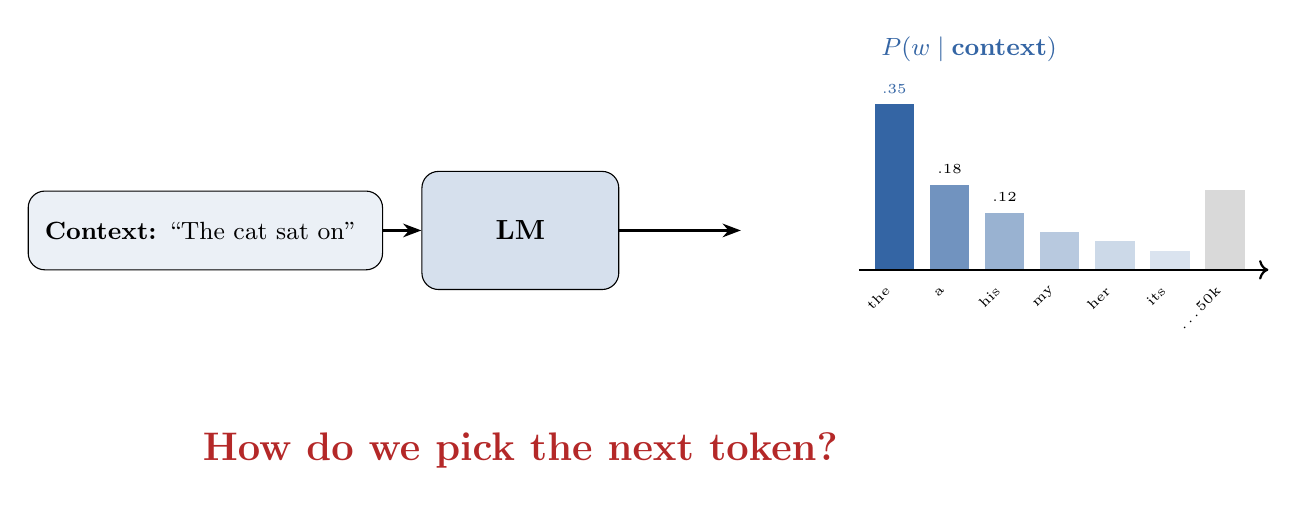
\begin{tikzpicture}[
  box/.style={draw, rounded corners=6pt, minimum height=1cm, align=center, font=\small}
]
  % Input tokens
  \node[box, fill=popblue!10, minimum width=4.5cm] (input) at (-4, 0) {
    \textbf{Context:} ``The cat sat on''
  };

  % Model box
  \node[box, fill=popblue!20, minimum width=2.5cm, minimum height=1.5cm, font=\normalsize\bfseries] (model) at (0, 0) {LM};

  % Arrow in
  \draw[-{Stealth}, thick] (input) -- (model);

  % Output: probability bars
  \begin{scope}[xshift=4.5cm, yshift=-0.5cm]
    \node[font=\small\bfseries, popblue] at (1.2, 2.8) {$P(w \mid \text{context})$};
    \fill[popblue]      (0,   0) rectangle (0.5, 2.1);
    \fill[popblue!70]   (0.7, 0) rectangle (1.2, 1.08);
    \fill[popblue!50]   (1.4, 0) rectangle (1.9, 0.72);
    \fill[popblue!35]   (2.1, 0) rectangle (2.6, 0.48);
    \fill[popblue!25]   (2.8, 0) rectangle (3.3, 0.36);
    \fill[popblue!18]   (3.5, 0) rectangle (4.0, 0.24);
    \fill[gray!30]      (4.2, 0) rectangle (4.7, 1.02);

    \node[font=\tiny, rotate=45, anchor=east] at (0.25, -0.15) {the};
    \node[font=\tiny, rotate=45, anchor=east] at (0.95, -0.15) {a};
    \node[font=\tiny, rotate=45, anchor=east] at (1.65, -0.15) {his};
    \node[font=\tiny, rotate=45, anchor=east] at (2.35, -0.15) {my};
    \node[font=\tiny, rotate=45, anchor=east] at (3.05, -0.15) {her};
    \node[font=\tiny, rotate=45, anchor=east] at (3.75, -0.15) {its};
    \node[font=\tiny, rotate=45, anchor=east] at (4.45, -0.15) {\ldots 50k};

    % Probability labels
    \node[font=\tiny, popblue] at (0.25, 2.3) {.35};
    \node[font=\tiny] at (0.95, 1.28) {.18};
    \node[font=\tiny] at (1.65, 0.92) {.12};

    \draw[thick, ->] (-0.2, 0) -- (5, 0);
  \end{scope}

  % Arrow out
  \draw[-{Stealth}, thick] (model) -- (2.8, 0);

  % Question
  \node[font=\Large\bfseries, text=warnred] at (0, -2.8) {How do we pick the next token?};
\end{tikzpicture}
\end{center}
\end{frame}

% ============================================================
% AUTOREGRESSIVE GENERATION
% ============================================================
\begin{frame}
\frametitle{Autoregressive generation}

\begin{center}
\vspace{-0.2cm}
$$P(w_1, w_2, \ldots, w_T) = \prod_{t=1}^{T} P\bigl(w_t \mid w_1, \ldots, w_{t-1}\bigr)$$
\end{center}

\vspace{0.2cm}
\begin{center}
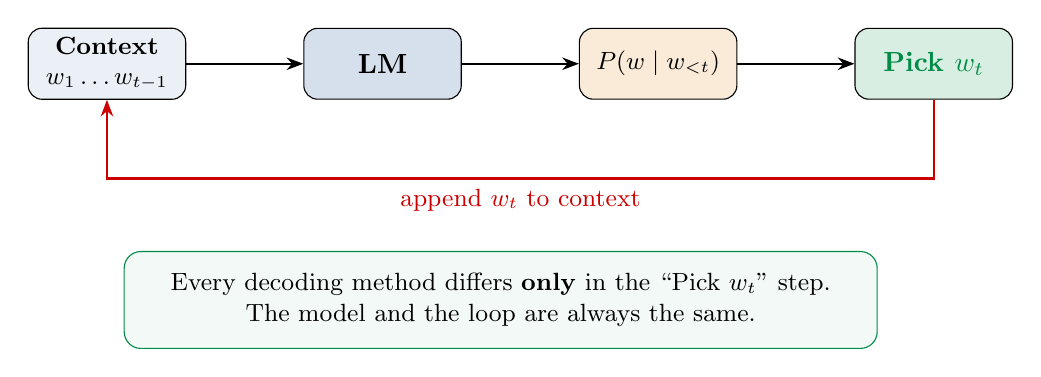
\begin{tikzpicture}[
  box/.style={draw, rounded corners=5pt, minimum height=0.9cm, minimum width=2cm, align=center, font=\small},
  arrow/.style={-{Stealth[length=6pt]}, thick}
]
  % Pipeline
  \node[box, fill=popblue!10] (ctx) at (-5, 0) {\textbf{Context}\\$w_1 \ldots w_{t-1}$};
  \node[box, fill=popblue!20, font=\normalsize\bfseries] (lm) at (-1.5, 0) {LM};
  \node[box, fill=orange1!15] (dist) at (2, 0) {$P(w \mid w_{<t})$};
  \node[box, fill=paramgreen!15, font=\normalsize\bfseries] (pick) at (5.5, 0) {\color{paramgreen}Pick $w_t$};

  \draw[arrow] (ctx) -- (lm);
  \draw[arrow] (lm) -- (dist);
  \draw[arrow] (dist) -- (pick);

  % Feedback loop
  \draw[arrow, sampred, thick] (pick.south) -- ++(0, -1) -| (ctx.south)
    node[pos=0.25, below, font=\small] {append $w_t$ to context};

  % Annotation
  \node[draw=paramgreen, fill=paramgreen!5, rounded corners=6pt, text width=9cm, align=center, inner sep=8pt, font=\small] at (0, -3) {
    Every decoding method differs \textbf{only} in the ``Pick $w_t$'' step.\\
    The model and the loop are always the same.
  };
\end{tikzpicture}
\end{center}
\end{frame}

% ============================================================
% GREEDY SEARCH
% ============================================================
\begin{frame}
\frametitle{Greedy search}

$$w_t = \arg\max_{w} \; P(w \mid w_1, \ldots, w_{t-1})$$

\vspace{0.1cm}
\begin{center}
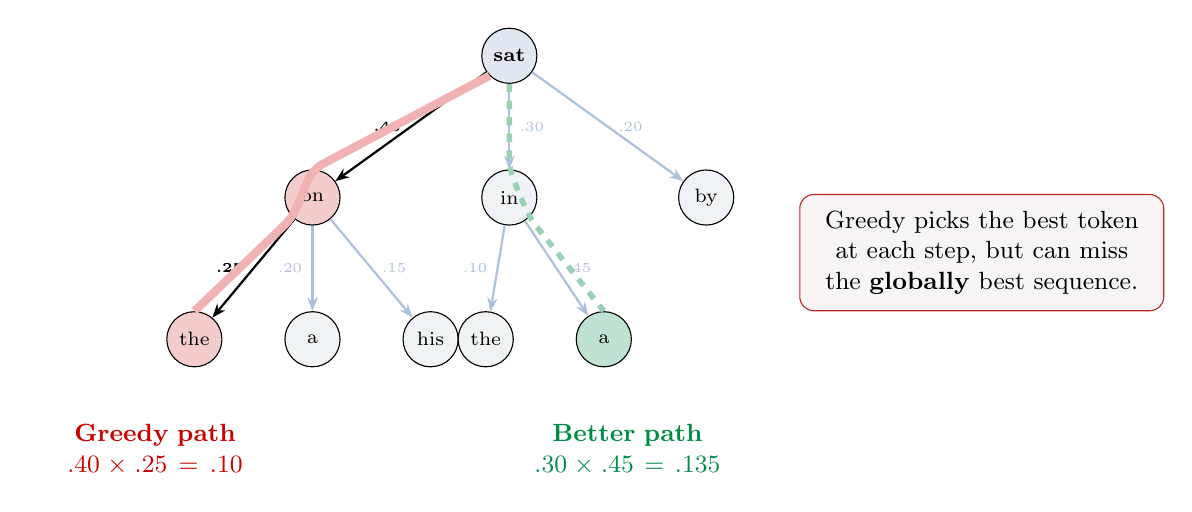
\begin{tikzpicture}[
  node/.style={draw, circle, minimum size=0.7cm, inner sep=0pt, font=\scriptsize},
  edge/.style={-{Stealth[length=5pt]}, thick},
  level distance=1.8cm,
  sibling distance=1.6cm
]
  % Root
  \node[node, fill=popblue!15] (root) at (0, 0) {\textbf{sat}};

  % Level 1
  \node[node, fill=sampred!20] (a) at (-2.5, -1.8) {on};
  \node[node, fill=popblue!8] (b) at (0, -1.8) {in};
  \node[node, fill=popblue!8] (c) at (2.5, -1.8) {by};

  \draw[edge] (root) -- (a) node[midway, left, font=\tiny] {\textbf{.40}};
  \draw[edge, popblue!40] (root) -- (b) node[midway, right, font=\tiny] {.30};
  \draw[edge, popblue!40] (root) -- (c) node[midway, right, font=\tiny] {.20};

  % Level 2 from "on"
  \node[node, fill=sampred!20] (a1) at (-4, -3.6) {the};
  \node[node, fill=popblue!8] (a2) at (-2.5, -3.6) {a};
  \node[node, fill=popblue!8] (a3) at (-1, -3.6) {his};

  \draw[edge] (a) -- (a1) node[midway, left, font=\tiny] {\textbf{.25}};
  \draw[edge, popblue!40] (a) -- (a2) node[midway, left, font=\tiny] {.20};
  \draw[edge, popblue!40] (a) -- (a3) node[midway, right, font=\tiny] {.15};

  % Level 2 from "in"
  \node[node, fill=popblue!8] (b1) at (-0.3, -3.6) {the};
  \node[node, fill=paramgreen!25] (b2) at (1.2, -3.6) {a};

  \draw[edge, popblue!40] (b) -- (b1) node[midway, left, font=\tiny] {.10};
  \draw[edge, popblue!40] (b) -- (b2) node[midway, right, font=\tiny] {.45};

  % Greedy path highlight
  \draw[line width=3pt, sampred!30, rounded corners]
    (root.south west) -- (a.north) -- (a.south west) -- (a1.north);

  % Best path highlight
  \draw[line width=2pt, paramgreen!40, rounded corners, dashed]
    (root.south) -- (b.north) -- (b.south east) -- (b2.north);

  % Annotations
  \node[font=\small, sampred, text width=3cm, align=center] at (-4.5, -5) {
    \textbf{Greedy path}\\$.40 \times .25 = .10$
  };
  \node[font=\small, paramgreen, text width=3cm, align=center] at (1.5, -5) {
    \textbf{Better path}\\$.30 \times .45 = .135$
  };

  % Right side annotation
  \node[draw=warnred, fill=warnred!5, rounded corners=5pt, text width=4.2cm, align=center, font=\small, inner sep=6pt] at (6, -2.5) {
    Greedy picks the best token\\at each step, but can miss\\the \textbf{globally} best sequence.
  };
\end{tikzpicture}
\end{center}
\end{frame}

% ============================================================
% GREEDY: THE REPETITION TRAP
% ============================================================
\begin{frame}
\frametitle{Greedy search: the repetition trap}

\begin{center}
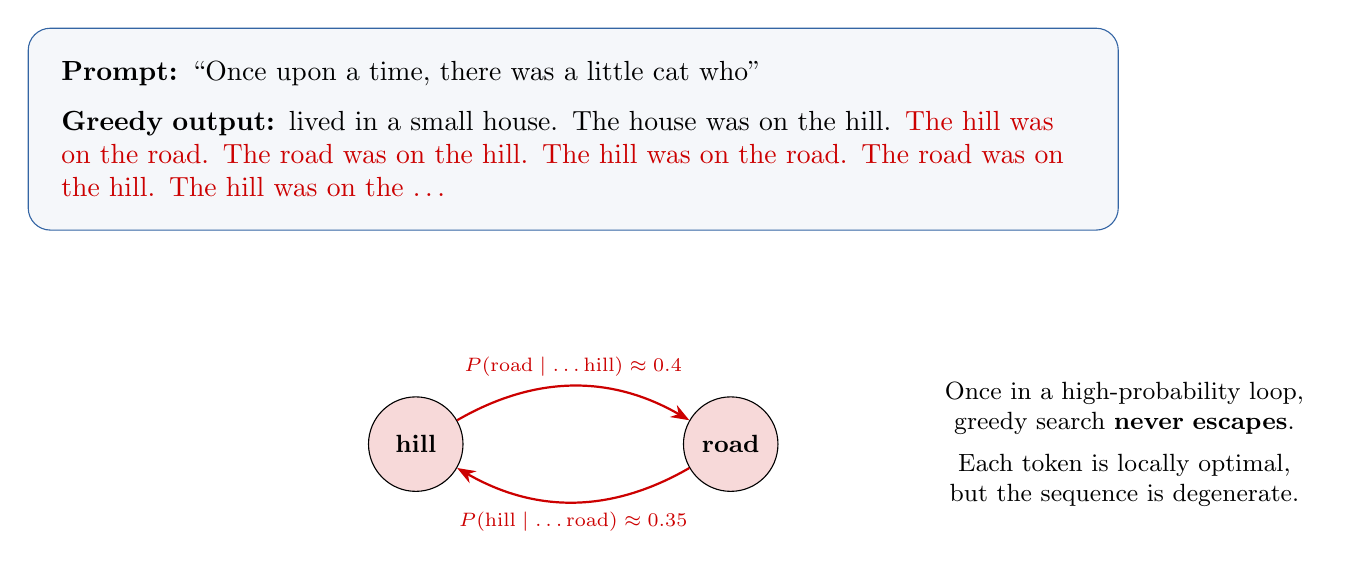
\begin{tikzpicture}
  % Generated text with fading repetition
  \node[draw=popblue, fill=popblue!5, rounded corners=8pt, text width=13cm, align=left, inner sep=12pt] at (0, 1.5) {
    \textbf{Prompt:} ``Once upon a time, there was a little cat who''\\[6pt]
    \textbf{Greedy output:} lived in a small house. The house was on the hill.
    {\color{sampred} The hill was on the road. The road was on the hill.
    The hill was on the road. The road was on the hill.
    The hill was on the \ldots}
  };

  % Cycle diagram
  \begin{scope}[yshift=-2.5cm]
    \node[draw, circle, fill=sampred!15, minimum size=1.2cm, font=\small\bfseries] (A) at (-2, 0) {hill};
    \node[draw, circle, fill=sampred!15, minimum size=1.2cm, font=\small\bfseries] (B) at (2, 0) {road};

    \draw[-{Stealth}, thick, sampred, bend left=30] (A) to node[above, font=\scriptsize] {$P(\text{road} \mid \ldots\text{hill}) \approx 0.4$} (B);
    \draw[-{Stealth}, thick, sampred, bend left=30] (B) to node[below, font=\scriptsize] {$P(\text{hill} \mid \ldots\text{road}) \approx 0.35$} (A);

    \node[font=\small, text width=5cm, align=center] at (7, 0) {
      Once in a high-probability loop,\\greedy search \textbf{never escapes}.\\[4pt]
      Each token is locally optimal,\\but the sequence is degenerate.
    };
  \end{scope}
\end{tikzpicture}
\end{center}
\end{frame}

% ============================================================
% BEAM SEARCH
% ============================================================
\begin{frame}
\frametitle{Beam search ($B = 2$)}

\begin{center}
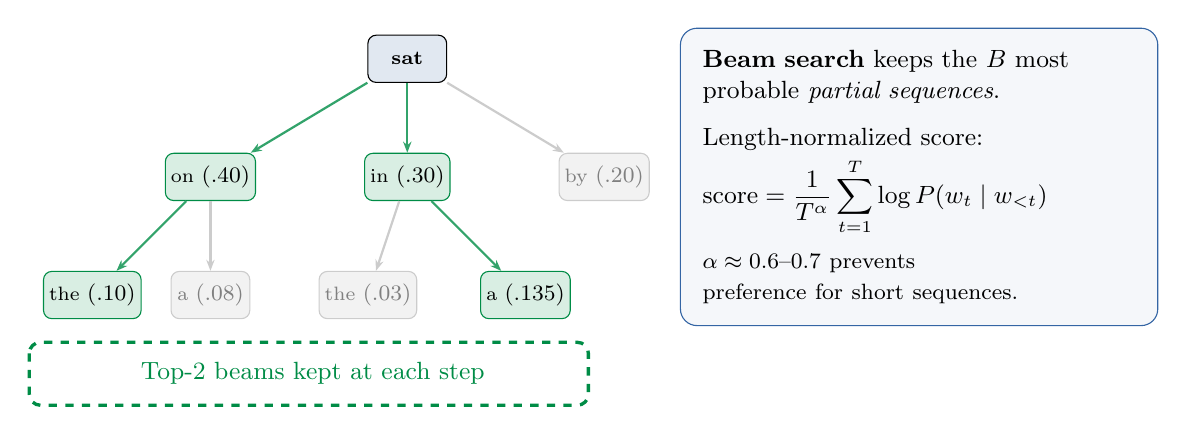
\begin{tikzpicture}[
  node/.style={draw, rounded corners=3pt, minimum width=1cm, minimum height=0.6cm, inner sep=2pt, font=\scriptsize, align=center},
  kept/.style={node, fill=paramgreen!15, draw=paramgreen},
  pruned/.style={node, fill=gray!10, draw=gray!40, text=gray},
  edge/.style={-{Stealth[length=4pt]}, thick},
  kedge/.style={edge, paramgreen!80},
  pedge/.style={edge, gray!40}
]
  % Start
  \node[node, fill=popblue!15] (start) at (0, 0) {\textbf{sat}};

  % Step 1
  \node[kept] (on) at (-2.5, -1.5) {on \footnotesize(.40)};
  \node[kept] (in) at (0, -1.5) {in \footnotesize(.30)};
  \node[pruned] (by) at (2.5, -1.5) {by \footnotesize(.20)};

  \draw[kedge] (start) -- (on);
  \draw[kedge] (start) -- (in);
  \draw[pedge] (start) -- (by);

  % Step 2 from "on"
  \node[kept] (on-the) at (-4, -3) {the \footnotesize(.10)};
  \node[pruned] (on-a) at (-2.5, -3) {a \footnotesize(.08)};

  \draw[kedge] (on) -- (on-the);
  \draw[pedge] (on) -- (on-a);

  % Step 2 from "in"
  \node[pruned] (in-the) at (-0.5, -3) {the \footnotesize(.03)};
  \node[kept] (in-a) at (1.5, -3) {a \footnotesize(.135)};

  \draw[pedge] (in) -- (in-the);
  \draw[kedge] (in) -- (in-a);

  % Final beams
  \draw[very thick, paramgreen, rounded corners, dashed]
    (-4.8, -3.6) rectangle (2.3, -4.4);
  \node[font=\small, paramgreen] at (-1.2, -4) {Top-2 beams kept at each step};

  % Legend / formula
  \node[draw=popblue, fill=popblue!5, rounded corners=6pt, text width=5.5cm, align=left, inner sep=8pt, font=\small] at (6.5, -1.5) {
    \textbf{Beam search} keeps the $B$ most\\
    probable \textit{partial sequences}.\\[6pt]
    Length-normalized score:\\[2pt]
    $\displaystyle \text{score} = \frac{1}{T^\alpha}\sum_{t=1}^{T} \log P(w_t \mid w_{<t})$\\[6pt]
    {\footnotesize $\alpha \approx 0.6$--$0.7$ prevents\\preference for short sequences.}
  };
\end{tikzpicture}
\end{center}
\end{frame}

% ============================================================
% BEAM SEARCH: TRADE-OFFS
% ============================================================
\begin{frame}
\frametitle{Beam search: trade-offs}

\begin{center}
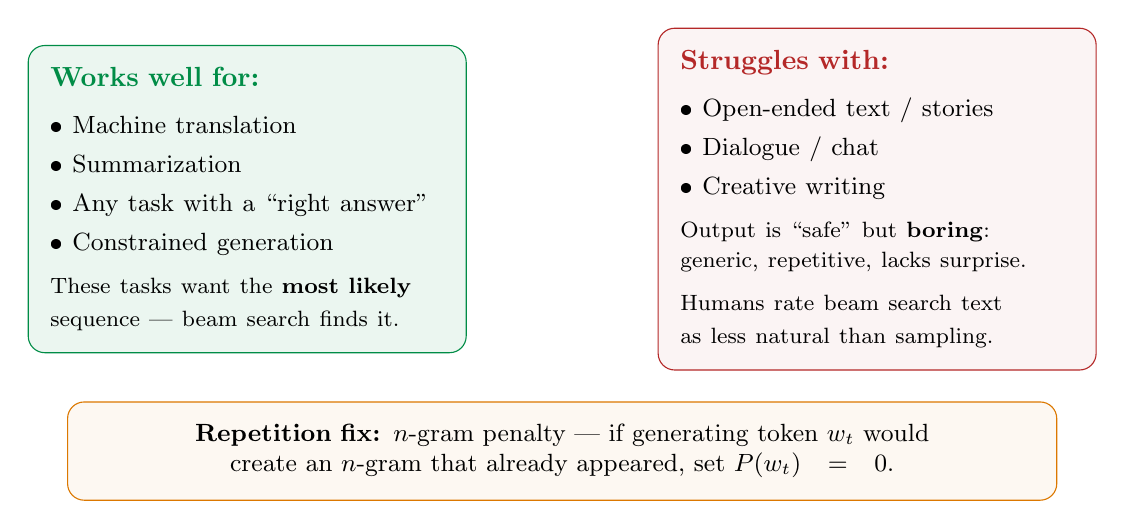
\begin{tikzpicture}[
  probox/.style={draw=paramgreen, fill=paramgreen!8, rounded corners=6pt, minimum width=5.5cm, minimum height=3.5cm, text width=5cm, align=left, inner sep=8pt},
  conbox/.style={draw=warnred, fill=warnred!5, rounded corners=6pt, minimum width=5.5cm, minimum height=3.5cm, text width=5cm, align=left, inner sep=8pt}
]
  \node[probox] at (-4, 0) {
    \textbf{\textcolor{paramgreen}{Works well for:}}\\[6pt]
    \small
    \textbullet\ Machine translation\\[3pt]
    \textbullet\ Summarization\\[3pt]
    \textbullet\ Any task with a ``right answer''\\[3pt]
    \textbullet\ Constrained generation\\[6pt]
    {\footnotesize These tasks want the \textbf{most likely}\\
    sequence --- beam search finds it.}
  };

  \node[conbox] at (4, 0) {
    \textbf{\textcolor{warnred}{Struggles with:}}\\[6pt]
    \small
    \textbullet\ Open-ended text / stories\\[3pt]
    \textbullet\ Dialogue / chat\\[3pt]
    \textbullet\ Creative writing\\[6pt]
    {\footnotesize Output is ``safe'' but \textbf{boring}:\\
    generic, repetitive, lacks surprise.}\\[6pt]
    {\footnotesize Humans rate beam search text\\as less natural than sampling.}
  };

  % N-gram trick
  \node[draw=orange1, fill=orange1!5, rounded corners=6pt, text width=12cm, align=center, inner sep=8pt, font=\small] at (0, -3.2) {
    \textbf{Repetition fix:} $n$-gram penalty --- if generating token $w_t$ would create an $n$-gram that already appeared, set $P(w_t) = 0$.
  };
\end{tikzpicture}
\end{center}
\end{frame}

% ============================================================
% THE PROBABILITY TRAP
% ============================================================
\begin{frame}
\frametitle{The probability trap}

\begin{center}
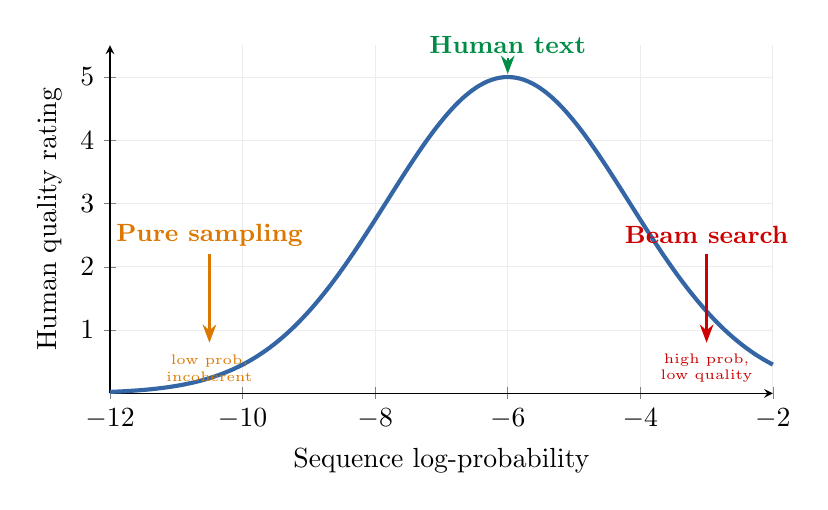
\begin{tikzpicture}
  \begin{axis}[
    width=10cm, height=6cm,
    xlabel={Sequence log-probability},
    ylabel={Human quality rating},
    xmin=-12, xmax=-2,
    ymin=0, ymax=5.5,
    axis lines=left,
    grid=major,
    grid style={gray!15},
    every axis plot/.append style={line width=1.5pt},
    xtick={-12,-10,-8,-6,-4,-2},
    ytick={1,2,3,4,5},
    clip=false
  ]
    % Quality curve (inverted U)
    \addplot[popblue, domain=-12:-2, samples=80, smooth]
      {5*exp(-0.15*(\x+6)^2)};

    % Annotations
    \node[font=\small\bfseries, sampred] at (axis cs:-3, 2.5) {Beam search};
    \draw[-{Stealth}, sampred, thick] (axis cs:-3, 2.2) -- (axis cs:-3, 0.8);
    \node[font=\tiny, sampred, text width=2cm, align=center] at (axis cs:-3, 0.4) {high prob,\\low quality};

    \node[font=\small\bfseries, paramgreen] at (axis cs:-6, 5.5) {Human text};
    \draw[-{Stealth}, paramgreen, thick] (axis cs:-6, 5.3) -- (axis cs:-6, 5.05);

    \node[font=\small\bfseries, orange1] at (axis cs:-10.5, 2.5) {Pure sampling};
    \draw[-{Stealth}, orange1, thick] (axis cs:-10.5, 2.2) -- (axis cs:-10.5, 0.8);
    \node[font=\tiny, orange1, text width=2cm, align=center] at (axis cs:-10.5, 0.4) {low prob,\\incoherent};
  \end{axis}
\end{tikzpicture}
\end{center}

\vspace{0.1cm}
\begin{center}
\fcolorbox{warnred}{warnred!5}{%
  \parbox{11cm}{\centering\small
    The highest-probability text is \textbf{not} the best text.\\
    Human language occupies a \textbf{sweet spot} of moderate probability.\\[2pt]
    {\footnotesize --- Holtzman et al., ``The Curious Case of Neural Text Degeneration'' (2019)}
  }%
}
\end{center}
\end{frame}

% ============================================================
% TEMPERATURE
% ============================================================
\begin{frame}
\frametitle{Temperature scaling}

$$p_i = \frac{\exp(z_i \,/\, T)}{\displaystyle\sum_{j} \exp(z_j \,/\, T)}$$

\vspace{0.1cm}
\begin{center}
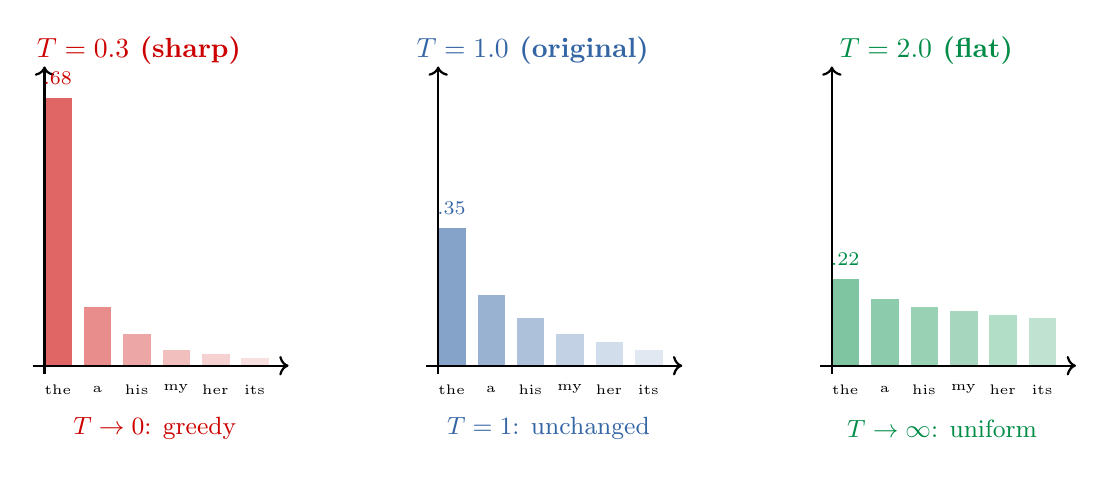
\begin{tikzpicture}
  % === T = 0.3 (sharp) ===
  \begin{scope}[xshift=-5cm]
    \node[font=\normalsize\bfseries, sampred] at (1.2, 4) {$T = 0.3$ (sharp)};
    \fill[sampred!60] (0, 0) rectangle (0.35, 3.4);
    \fill[sampred!45] (0.5, 0) rectangle (0.85, 0.75);
    \fill[sampred!35] (1.0, 0) rectangle (1.35, 0.4);
    \fill[sampred!25] (1.5, 0) rectangle (1.85, 0.2);
    \fill[sampred!18] (2.0, 0) rectangle (2.35, 0.15);
    \fill[sampred!12] (2.5, 0) rectangle (2.85, 0.1);
    \draw[thick, ->] (-0.15, 0) -- (3.1, 0);
    \draw[thick, ->] (0, -0.1) -- (0, 3.8);
    \node[font=\tiny] at (0.17, -0.3) {the};
    \node[font=\tiny] at (0.67, -0.3) {a};
    \node[font=\tiny] at (1.17, -0.3) {his};
    \node[font=\tiny] at (1.67, -0.3) {my};
    \node[font=\tiny] at (2.17, -0.3) {her};
    \node[font=\tiny] at (2.67, -0.3) {its};
    \node[font=\scriptsize, sampred] at (0.17, 3.65) {.68};
    \node[font=\small, sampred] at (1.4, -0.8) {$T \to 0$: greedy};
  \end{scope}

  % === T = 1.0 (original) ===
  \begin{scope}[xshift=0cm]
    \node[font=\normalsize\bfseries, popblue] at (1.2, 4) {$T = 1.0$ (original)};
    \fill[popblue!60] (0, 0) rectangle (0.35, 1.75);
    \fill[popblue!50] (0.5, 0) rectangle (0.85, 0.9);
    \fill[popblue!40] (1.0, 0) rectangle (1.35, 0.6);
    \fill[popblue!30] (1.5, 0) rectangle (1.85, 0.4);
    \fill[popblue!22] (2.0, 0) rectangle (2.35, 0.3);
    \fill[popblue!15] (2.5, 0) rectangle (2.85, 0.2);
    \draw[thick, ->] (-0.15, 0) -- (3.1, 0);
    \draw[thick, ->] (0, -0.1) -- (0, 3.8);
    \node[font=\tiny] at (0.17, -0.3) {the};
    \node[font=\tiny] at (0.67, -0.3) {a};
    \node[font=\tiny] at (1.17, -0.3) {his};
    \node[font=\tiny] at (1.67, -0.3) {my};
    \node[font=\tiny] at (2.17, -0.3) {her};
    \node[font=\tiny] at (2.67, -0.3) {its};
    \node[font=\scriptsize, popblue] at (0.17, 2.0) {.35};
    \node[font=\small, popblue] at (1.4, -0.8) {$T = 1$: unchanged};
  \end{scope}

  % === T = 2.0 (flat) ===
  \begin{scope}[xshift=5cm]
    \node[font=\normalsize\bfseries, paramgreen] at (1.2, 4) {$T = 2.0$ (flat)};
    \fill[paramgreen!50] (0, 0) rectangle (0.35, 1.1);
    \fill[paramgreen!45] (0.5, 0) rectangle (0.85, 0.85);
    \fill[paramgreen!40] (1.0, 0) rectangle (1.35, 0.75);
    \fill[paramgreen!35] (1.5, 0) rectangle (1.85, 0.7);
    \fill[paramgreen!30] (2.0, 0) rectangle (2.35, 0.65);
    \fill[paramgreen!25] (2.5, 0) rectangle (2.85, 0.6);
    \draw[thick, ->] (-0.15, 0) -- (3.1, 0);
    \draw[thick, ->] (0, -0.1) -- (0, 3.8);
    \node[font=\tiny] at (0.17, -0.3) {the};
    \node[font=\tiny] at (0.67, -0.3) {a};
    \node[font=\tiny] at (1.17, -0.3) {his};
    \node[font=\tiny] at (1.67, -0.3) {my};
    \node[font=\tiny] at (2.17, -0.3) {her};
    \node[font=\tiny] at (2.67, -0.3) {its};
    \node[font=\scriptsize, paramgreen] at (0.17, 1.35) {.22};
    \node[font=\small, paramgreen] at (1.4, -0.8) {$T \to \infty$: uniform};
  \end{scope}
\end{tikzpicture}
\end{center}

\vspace{0.2cm}
\begin{center}
{\small Temperature \textbf{reshapes} the distribution --- lower $=$ more focused, higher $=$ more random.}
\end{center}
\end{frame}

% ============================================================
% SAMPLING
% ============================================================
\begin{frame}
\frametitle{Sampling from the distribution}

$$w_t \sim P(\cdot \mid w_1, \ldots, w_{t-1})$$

\vspace{0.2cm}
\begin{center}
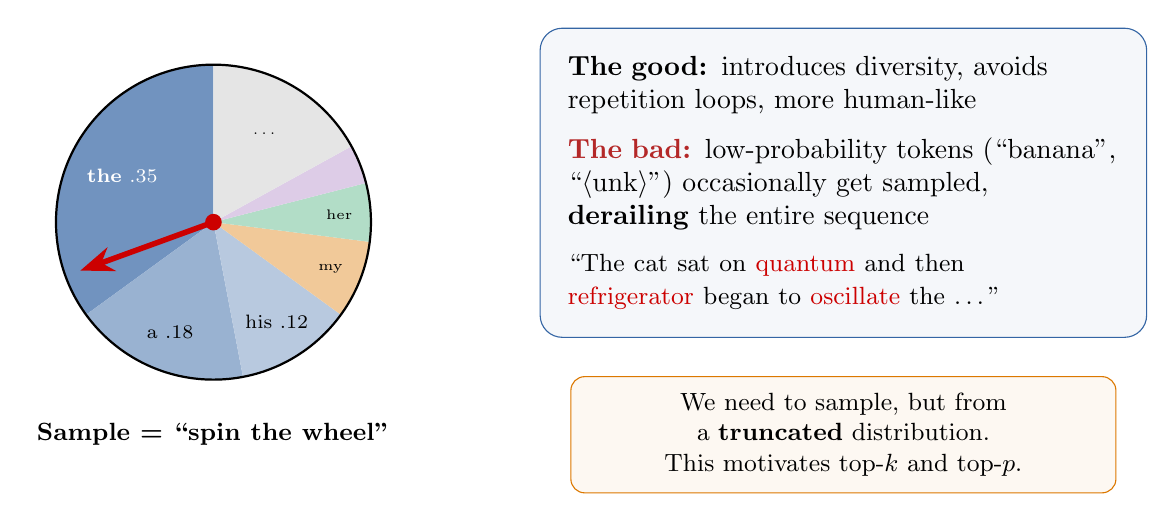
\begin{tikzpicture}
  % Probability wheel
  \begin{scope}[xshift=-3.5cm]
    % Pie chart
    \fill[popblue!70] (0,0) -- (90:2) arc (90:90+126:2) -- cycle;     % the: 0.35
    \fill[popblue!50] (0,0) -- (216:2) arc (216:216+64.8:2) -- cycle;  % a: 0.18
    \fill[popblue!35] (0,0) -- (280.8:2) arc (280.8:280.8+43.2:2) -- cycle; % his: 0.12
    \fill[orange1!40] (0,0) -- (324:2) arc (324:324+28.8:2) -- cycle;  % my: 0.08
    \fill[paramgreen!30] (0,0) -- (352.8:2) arc (352.8:352.8+21.6:2) -- cycle; % her: 0.06
    \fill[violet1!25] (0,0) -- (14.4:2) arc (14.4:14.4+14.4:2) -- cycle; % its: 0.04
    \fill[gray!20] (0,0) -- (28.8:2) arc (28.8:90:2) -- cycle;         % rest: 0.17

    \draw[thick] (0,0) circle (2);

    % Labels
    \node[font=\scriptsize, white] at (153:1.3) {\textbf{the} .35};
    \node[font=\scriptsize] at (248.4:1.5) {a .18};
    \node[font=\scriptsize] at (302.4:1.5) {his .12};
    \node[font=\tiny] at (338.4:1.6) {my};
    \node[font=\tiny] at (3.6:1.6) {her};
    \node[font=\tiny] at (59.4:1.3) {\ldots};

    % Spinner arrow
    \draw[-{Stealth}, very thick, sampred, line width=2pt] (0,0) -- (200:1.8);
    \fill[sampred] (0,0) circle (3pt);

    \node[font=\small\bfseries] at (0, -2.7) {Sample = ``spin the wheel''};
  \end{scope}

  % Problem illustration
  \begin{scope}[xshift=4.5cm]
    \node[draw=popblue, fill=popblue!5, rounded corners=8pt, text width=7cm, align=left, inner sep=10pt] at (0, 0.5) {
      \textbf{The good:} introduces diversity, avoids\\repetition loops, more human-like\\[6pt]
      \textbf{\textcolor{warnred}{The bad:}} low-probability tokens (``banana'',\\``$\langle$unk$\rangle$'') occasionally get sampled,\\
      \textbf{derailing} the entire sequence\\[6pt]
      {\small ``The cat sat on \textcolor{sampred}{quantum} and then\\
      \textcolor{sampred}{refrigerator} began to \textcolor{sampred}{oscillate} the \ldots''}
    };

    \node[draw=orange1, fill=orange1!5, rounded corners=5pt, text width=6.5cm, align=center, inner sep=6pt, font=\small] at (0, -2.7) {
      We need to sample, but from a \textbf{truncated} distribution.\\
      This motivates top-$k$ and top-$p$.
    };
  \end{scope}
\end{tikzpicture}
\end{center}
\end{frame}

% ============================================================
% TOP-K SAMPLING
% ============================================================
\begin{frame}
\frametitle{Top-$k$ sampling}

\textbf{Idea:} Keep only the $k$ most probable tokens, zero out the rest, renormalize.

\vspace{0.3cm}
\begin{center}
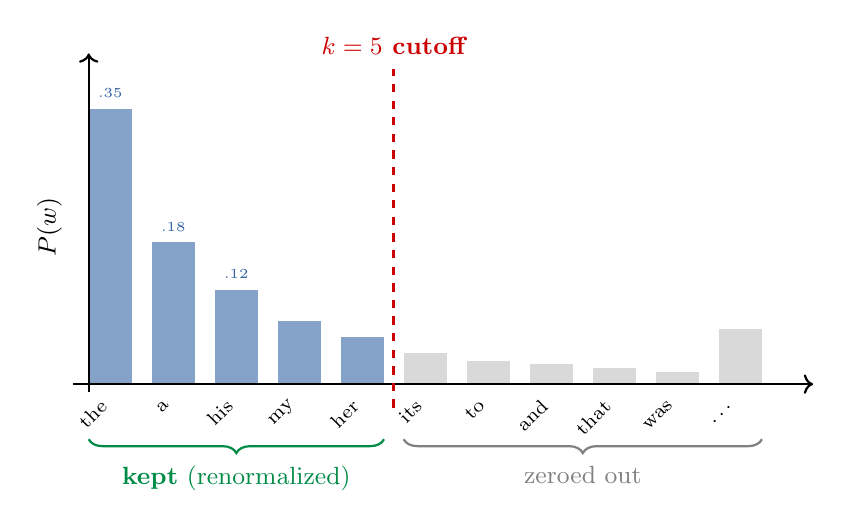
\begin{tikzpicture}
  % Bar chart with cutoff (manual TikZ bars)
  \def\bw{0.55}  % bar width
  \def\sp{0.8}   % bar spacing

  % Kept bars (green tint)
  \fill[popblue!60] (0*\sp, 0) rectangle (0*\sp+\bw, 3.5);       % the: 0.35
  \fill[popblue!60] (1*\sp, 0) rectangle (1*\sp+\bw, 1.8);       % a: 0.18
  \fill[popblue!60] (2*\sp, 0) rectangle (2*\sp+\bw, 1.2);       % his: 0.12
  \fill[popblue!60] (3*\sp, 0) rectangle (3*\sp+\bw, 0.8);       % my: 0.08
  \fill[popblue!60] (4*\sp, 0) rectangle (4*\sp+\bw, 0.6);       % her: 0.06

  % Zeroed bars (gray)
  \fill[gray!30] (5*\sp, 0) rectangle (5*\sp+\bw, 0.4);          % its: 0.04
  \fill[gray!30] (6*\sp, 0) rectangle (6*\sp+\bw, 0.3);          % to: 0.03
  \fill[gray!30] (7*\sp, 0) rectangle (7*\sp+\bw, 0.25);         % and: 0.025
  \fill[gray!30] (8*\sp, 0) rectangle (8*\sp+\bw, 0.2);          % that: 0.02
  \fill[gray!30] (9*\sp, 0) rectangle (9*\sp+\bw, 0.15);         % was: 0.015
  \fill[gray!30] (10*\sp, 0) rectangle (10*\sp+\bw, 0.7);        % ...: rest

  % Axes
  \draw[thick, ->] (-0.2, 0) -- (9.2, 0);
  \draw[thick, ->] (0, -0.1) -- (0, 4.2);
  \node[font=\small, rotate=90] at (-0.5, 2) {$P(w)$};

  % Labels
  \foreach \i/\w in {0/the, 1/a, 2/his, 3/my, 4/her, 5/its, 6/to, 7/and, 8/that, 9/was, 10/{\ldots}} {
    \node[font=\scriptsize, rotate=45, anchor=east] at (\i*\sp+\bw/2, -0.15) {\w};
  }

  % Prob labels on top bars
  \node[font=\tiny, popblue] at (0*\sp+\bw/2, 3.7) {.35};
  \node[font=\tiny, popblue] at (1*\sp+\bw/2, 2.0) {.18};
  \node[font=\tiny, popblue] at (2*\sp+\bw/2, 1.4) {.12};

  % Cutoff line
  \draw[very thick, sampred, dashed] (4*\sp+\bw+0.12, -0.3) -- (4*\sp+\bw+0.12, 4.0);
  \node[font=\small\bfseries, sampred] at (4*\sp+\bw+0.12, 4.3) {$k = 5$ cutoff};

  % Braces
  \draw[thick, paramgreen, decorate, decoration={brace, amplitude=5pt, mirror}]
    (0, -0.7) -- (4*\sp+\bw, -0.7)
    node[midway, below=6pt, font=\small, paramgreen] {\textbf{kept} (renormalized)};

  \draw[thick, gray, decorate, decoration={brace, amplitude=5pt, mirror}]
    (5*\sp, -0.7) -- (10*\sp+\bw, -0.7)
    node[midway, below=6pt, font=\small, gray] {zeroed out};
\end{tikzpicture}
\end{center}

\vspace{0.1cm}
\begin{center}
\fcolorbox{warnred}{warnred!5}{%
  \parbox{11cm}{\centering\small
    \textbf{Problem:} Fixed $k$ doesn't adapt.
    When the model is \textbf{confident}, $k{=}50$ includes garbage.
    When the model is \textbf{uncertain}, $k{=}10$ cuts off good options.
  }%
}
\end{center}
\end{frame}

% ============================================================
% TOP-P (NUCLEUS) SAMPLING
% ============================================================
\begin{frame}
\frametitle{Top-$p$ (nucleus) sampling}

\textbf{Idea:} Find the smallest set $V_p$ such that $\displaystyle\sum_{w \in V_p} P(w) \ge p$.

\vspace{0.2cm}
\begin{center}
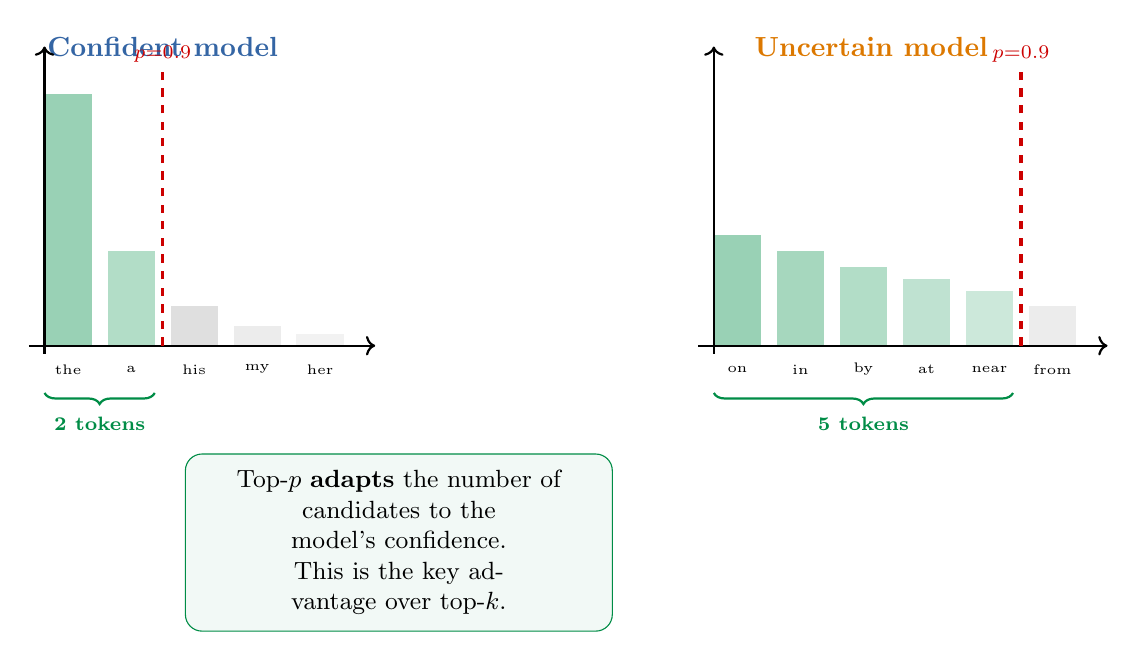
\begin{tikzpicture}
  % LEFT: Peaked distribution
  \begin{scope}[xshift=-4.5cm]
    \node[font=\normalsize\bfseries, popblue] at (1.5, 3.8) {Confident model};

    \fill[paramgreen!40] (0, 0) rectangle (0.6, 3.2);
    \fill[paramgreen!30] (0.8, 0) rectangle (1.4, 1.2);
    \fill[gray!25] (1.6, 0) rectangle (2.2, 0.5);
    \fill[gray!15] (2.4, 0) rectangle (3.0, 0.25);
    \fill[gray!10] (3.2, 0) rectangle (3.8, 0.15);

    \draw[thick, ->] (-0.2, 0) -- (4.2, 0);
    \draw[thick, ->] (0, -0.1) -- (0, 3.8);

    \node[font=\tiny] at (0.3, -0.3) {the};
    \node[font=\tiny] at (1.1, -0.3) {a};
    \node[font=\tiny] at (1.9, -0.3) {his};
    \node[font=\tiny] at (2.7, -0.3) {my};
    \node[font=\tiny] at (3.5, -0.3) {her};

    % Cumulative threshold line
    \draw[very thick, sampred, dashed] (1.5, 0) -- (1.5, 3.5);
    \node[font=\scriptsize, sampred] at (1.5, 3.7) {$p{=}0.9$};

    % Bracket
    \draw[thick, paramgreen, decorate, decoration={brace, amplitude=4pt, mirror}]
      (0, -0.6) -- (1.4, -0.6)
      node[midway, below=5pt, font=\scriptsize, paramgreen] {\textbf{2 tokens}};
  \end{scope}

  % RIGHT: Flat distribution
  \begin{scope}[xshift=4cm]
    \node[font=\normalsize\bfseries, orange1] at (2, 3.8) {Uncertain model};

    \fill[paramgreen!40] (0, 0) rectangle (0.6, 1.4);
    \fill[paramgreen!35] (0.8, 0) rectangle (1.4, 1.2);
    \fill[paramgreen!30] (1.6, 0) rectangle (2.2, 1.0);
    \fill[paramgreen!25] (2.4, 0) rectangle (3.0, 0.85);
    \fill[paramgreen!20] (3.2, 0) rectangle (3.8, 0.7);
    \fill[gray!15] (4.0, 0) rectangle (4.6, 0.5);

    \draw[thick, ->] (-0.2, 0) -- (5, 0);
    \draw[thick, ->] (0, -0.1) -- (0, 3.8);

    \node[font=\tiny] at (0.3, -0.3) {on};
    \node[font=\tiny] at (1.1, -0.3) {in};
    \node[font=\tiny] at (1.9, -0.3) {by};
    \node[font=\tiny] at (2.7, -0.3) {at};
    \node[font=\tiny] at (3.5, -0.3) {near};
    \node[font=\tiny] at (4.3, -0.3) {from};

    % Cumulative threshold line
    \draw[very thick, sampred, dashed] (3.9, 0) -- (3.9, 3.5);
    \node[font=\scriptsize, sampred] at (3.9, 3.7) {$p{=}0.9$};

    % Bracket
    \draw[thick, paramgreen, decorate, decoration={brace, amplitude=4pt, mirror}]
      (0, -0.6) -- (3.8, -0.6)
      node[midway, below=5pt, font=\scriptsize, paramgreen] {\textbf{5 tokens}};
  \end{scope}

  % Center annotation
  \node[draw=paramgreen, fill=paramgreen!5, rounded corners=6pt, text width=5cm, align=center, inner sep=6pt, font=\small] at (0, -2.5) {
    Top-$p$ \textbf{adapts} the number of\\
    candidates to the model's confidence.\\
    This is the key advantage over top-$k$.
  };
\end{tikzpicture}
\end{center}
\end{frame}

% ============================================================
% COMBINING: TEMPERATURE + TOP-P
% ============================================================
\begin{frame}
\frametitle{Combining the knobs}

\begin{center}
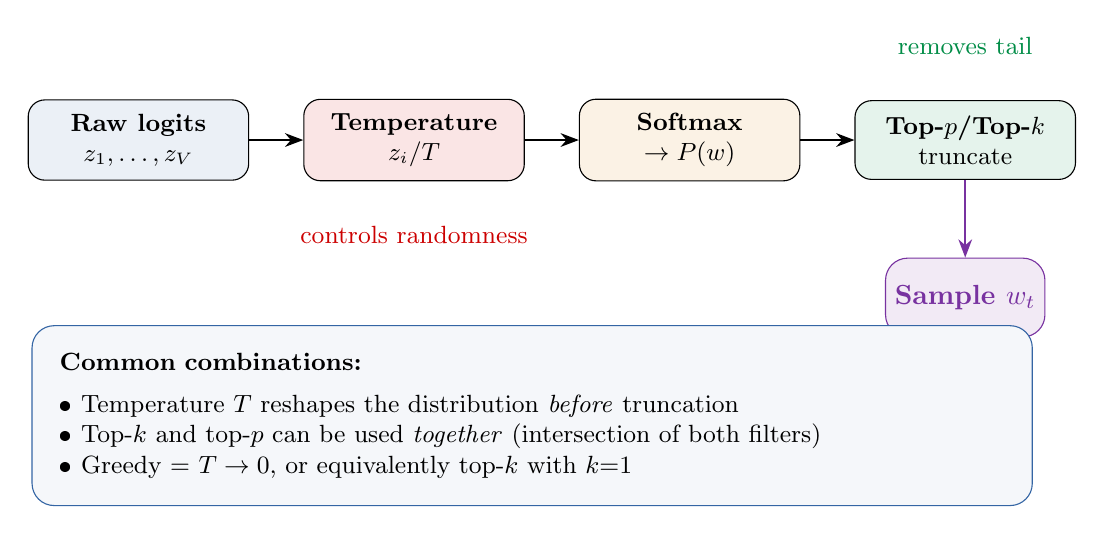
\begin{tikzpicture}[
  box/.style={draw, rounded corners=6pt, minimum width=2.8cm, minimum height=1cm, align=center, font=\small, inner sep=5pt}
]
  % Pipeline
  \node[box, fill=popblue!10] (logits) at (-5, 0) {\textbf{Raw logits}\\$z_1, \ldots, z_V$};
  \node[box, fill=sampred!10] (temp) at (-1.5, 0) {\textbf{Temperature}\\$z_i / T$};
  \node[box, fill=orange1!10] (softmax) at (2, 0) {\textbf{Softmax}\\$\to P(w)$};
  \node[box, fill=paramgreen!10] (trunc) at (5.5, 0) {\textbf{Top-$p$/Top-$k$}\\truncate};

  \draw[-{Stealth}, thick] (logits) -- (temp);
  \draw[-{Stealth}, thick] (temp) -- (softmax);
  \draw[-{Stealth}, thick] (softmax) -- (trunc);

  % Sample
  \node[draw=violet1, fill=violet1!10, rounded corners=8pt, minimum width=2cm, minimum height=1cm, font=\normalsize\bfseries] (sample) at (5.5, -2) {\color{violet1}Sample $w_t$};
  \draw[-{Stealth}, thick, violet1] (trunc) -- (sample);

  % Annotations
  \node[font=\small, text=sampred] at (-1.5, -1.2) {controls randomness};
  \node[font=\small, text=paramgreen] at (5.5, 1.2) {removes tail};

  % Common combos
  \node[draw=popblue, fill=popblue!5, rounded corners=8pt, text width=12cm, align=left, inner sep=10pt, font=\small] at (0, -3.5) {
    \textbf{Common combinations:}\\[4pt]
    \textbullet\ Temperature $T$ reshapes the distribution \textit{before} truncation\\
    \textbullet\ Top-$k$ and top-$p$ can be used \textit{together} (intersection of both filters)\\
    \textbullet\ Greedy = $T \to 0$, or equivalently top-$k$ with $k{=}1$
  };
\end{tikzpicture}
\end{center}
\end{frame}

% ============================================================
% COMPARISON TABLE
% ============================================================
\begin{frame}
\frametitle{Comparison of decoding strategies}

\vspace{-0.1cm}
\renewcommand{\arraystretch}{1.6}
\begin{center}
\begin{tabular}{>{\bfseries}l c c c}
  \textbf{Method} & \textbf{Deterministic?} & \textbf{Best for} & \textbf{Main weakness} \\
  \hline
  \textcolor{popblue}{Greedy} & Yes & Quick baseline & Repetitive, local optima \\[2pt]
  \textcolor{popblue}{Beam search} & Yes & Translation, summary & ``Boring'' open-ended text \\[2pt]
  \textcolor{sampred}{Temperature} & --- & \textit{Modifier, not standalone} & Just a knob \\[2pt]
  \textcolor{orange1}{Top-$k$} & No & Open-ended generation & Fixed $k$ doesn't adapt \\[2pt]
  \textcolor{paramgreen}{Top-$p$} & No & Open-ended generation & Slightly slower than top-$k$ \\
  \hline
\end{tabular}
\end{center}

\vspace{0.4cm}
\begin{center}
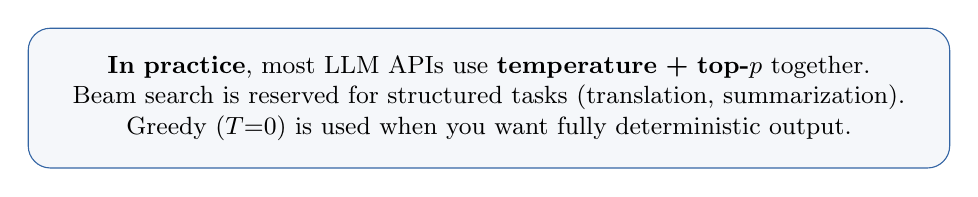
\begin{tikzpicture}
  \node[draw=popblue, fill=popblue!5, rounded corners=8pt, text width=11cm, align=center, inner sep=10pt, font=\small] {
    \textbf{In practice}, most LLM APIs use \textbf{temperature + top-$p$} together.\\
    Beam search is reserved for structured tasks (translation, summarization).\\
    Greedy ($T{=}0$) is used when you want fully deterministic output.
  };
\end{tikzpicture}
\end{center}
\end{frame}

% ============================================================
% PRACTICAL: API PARAMETERS
% ============================================================
\begin{frame}
\frametitle{Practical: typical API parameters}

\begin{center}
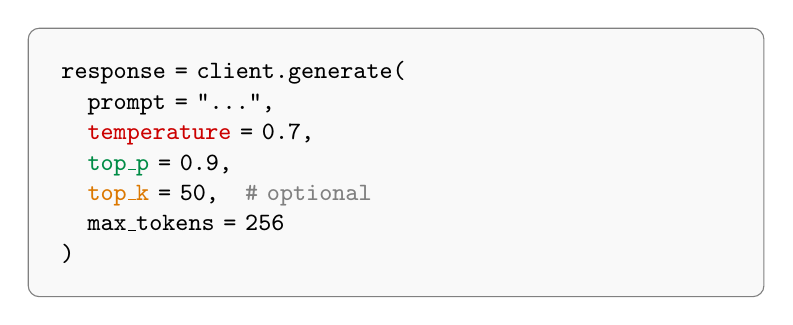
\begin{tikzpicture}
  % Code-like box
  \node[draw=gray, fill=gray!5, rounded corners=4pt, text width=8.5cm, align=left, inner sep=12pt, font=\ttfamily\small] at (0, 1.5) {
    response = client.generate(\\
    \quad prompt = "...",\\
    \quad \textcolor{sampred}{temperature} = 0.7,\\
    \quad \textcolor{paramgreen}{top\_p} = 0.9,\\
    \quad \textcolor{orange1}{top\_k} = 50,\quad\textcolor{gray}{\# optional}\\
    \quad max\_tokens = 256\\
    )
  };
\end{tikzpicture}
\end{center}

\vspace{0.2cm}
\begin{center}
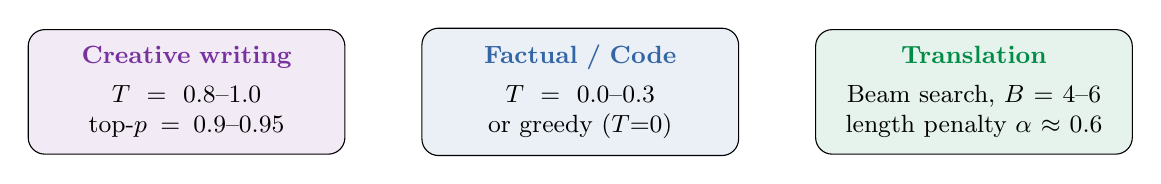
\begin{tikzpicture}[
  recbox/.style={draw, rounded corners=6pt, minimum width=4cm, minimum height=1.5cm, text width=3.6cm, align=center, inner sep=6pt, font=\small}
]
  \node[recbox, fill=violet1!10] at (-5, 0) {
    \textbf{\textcolor{violet1}{Creative writing}}\\[3pt]
    $T = 0.8$--$1.0$\\
    top-$p = 0.9$--$0.95$
  };
  \node[recbox, fill=popblue!10] at (0, 0) {
    \textbf{\textcolor{popblue}{Factual / Code}}\\[3pt]
    $T = 0.0$--$0.3$\\
    or greedy ($T{=}0$)
  };
  \node[recbox, fill=paramgreen!10] at (5, 0) {
    \textbf{\textcolor{paramgreen}{Translation}}\\[3pt]
    Beam search, $B = 4$--$6$\\
    length penalty $\alpha \approx 0.6$
  };
\end{tikzpicture}
\end{center}
\end{frame}

% ============================================================
% QUESTIONS
% ============================================================
\begin{frame}
\begin{center}
  {\Huge\bfseries\textcolor{popblue}{Questions?}}

  \vspace{1cm}

  {\large Next: Evaluation --- Perplexity, BLEU, ROUGE}
\end{center}
\end{frame}

\end{document}
